%mainfile: ../master.tex
\section{Events}\label{sec:events}

\citet{OOAD} defines an event as: \enquote{An instantanious event that involves one or more objects}. By understanding which events can happen in the problem domain, the behaviour of objects in the problem domain can be understood, further understanding possible usecases of the system.

The events in \cref{tab:eventtable}, only shows some possible events, that can take place in the problem domain. There are however infinitely many events that can happen, as an event can be identified as observable changes of sensor values. When choosing the events, the focus was on the events being representative of all possible events.

A short clarification of the chosen examples of events can be seen in the following paragraphs.

\paragraph{Enter/leave room} A person enters or leaves a room in the problem domain i.e. the automated home.
\paragraph{Turn on/off appliance} A person has turned on or off an appliance in the home.
\paragraph{Changes in external light} The light intensity outside of the home changes e.g. the sun rises.
\paragraph{Watching TV} A person is inactive and watching the activated TV.

\begin{table}
  \centering
  \begin{tabular}{*{7}{|l}|}
    \hline
    Event & Person & Action & State & Pattern & Location & Time \\
    \hline
    Enter/leave room & \checkmark & \checkmark & \checkmark & \checkmark & \checkmark & \checkmark\\
    \hline
    Turn on/off appliance & \checkmark & \checkmark & \checkmark & \checkmark & & \checkmark\\
    \hline
    Changes in external light & & & \checkmark & \checkmark & & \checkmark\\
    \hline
    Watching TV & \checkmark & \checkmark & & \checkmark & & \checkmark\\
    \hline
  \end{tabular}
  \caption{Event table}
  \label{tab:eventtable}
\end{table}
% \begin{table}[h!]
%   \centering
%   \begin{adjustbox}{max width=\textwidth}
%     \begin{tabular}{*{8}{|l}|}
%         \hline
%         \textbf{Event}                     & Person & Action & State & Pattern & Sensor & Actuator & Location & Time   \\
%         \hline
%         User entered lo0cation (unexpected) & \cmark & \cmark & \cmark  & \cmark   & \cmark   & \cmark & \cmark   & \cmark   & \cmark \\
%         \hline
%         User entered location (expected)   & \cmark & \cmark & \cmark  & \cmark   & \cmark   & \cmark & \cmark   & \cmark   & \cmark \\
%         \hline
%         Left home & \cmark & \cmark & \cmark & & \cmark & & \cmark & & \cmark & \cmark & \\
%         \hline
%         Enter room & \cmark & \cmark & \cmark & & \cmark & & \cmark & \cmark & \cmark & & \\
%         \hline
%         Left room & \cmark & \cmark & \cmark & & \cmark & & \cmark & \cmark & \cmark & &\\
%         \hline
%         Flicked switch & \cmark & \cmark & \cmark & \cmark & \cmark & \cmark & \cmark & \cmark & \cmark & & \\
%         \hline
%         Outside/External light intensity down & \cmark & & & & \cmark & \cmark & \cmark & \cmark & \cmark & &\\
%         \hline
%         Outside/External light intensity up & \cmark & & & & \cmark & \cmark & \cmark & \cmark& \cmark & &\\
%         \hline
%         Person sleeping & \cmark & \cmark & \cmark & & \cmark & & \cmark & & \cmark & & \cmark\\
%         \hline
%     \end{tabular}
%   \end{adjustbox}
%   \caption{Event table}
%   \label{tab:eventtable}
% \end{table}

\sinote{Udkommenteret i Tex dokument, er et behaviour diagram. Hvad skal det bruges til?}
% \begin{figure}
%    \centering
%    \begin{adjustbox}{max width=\textwidth}
%     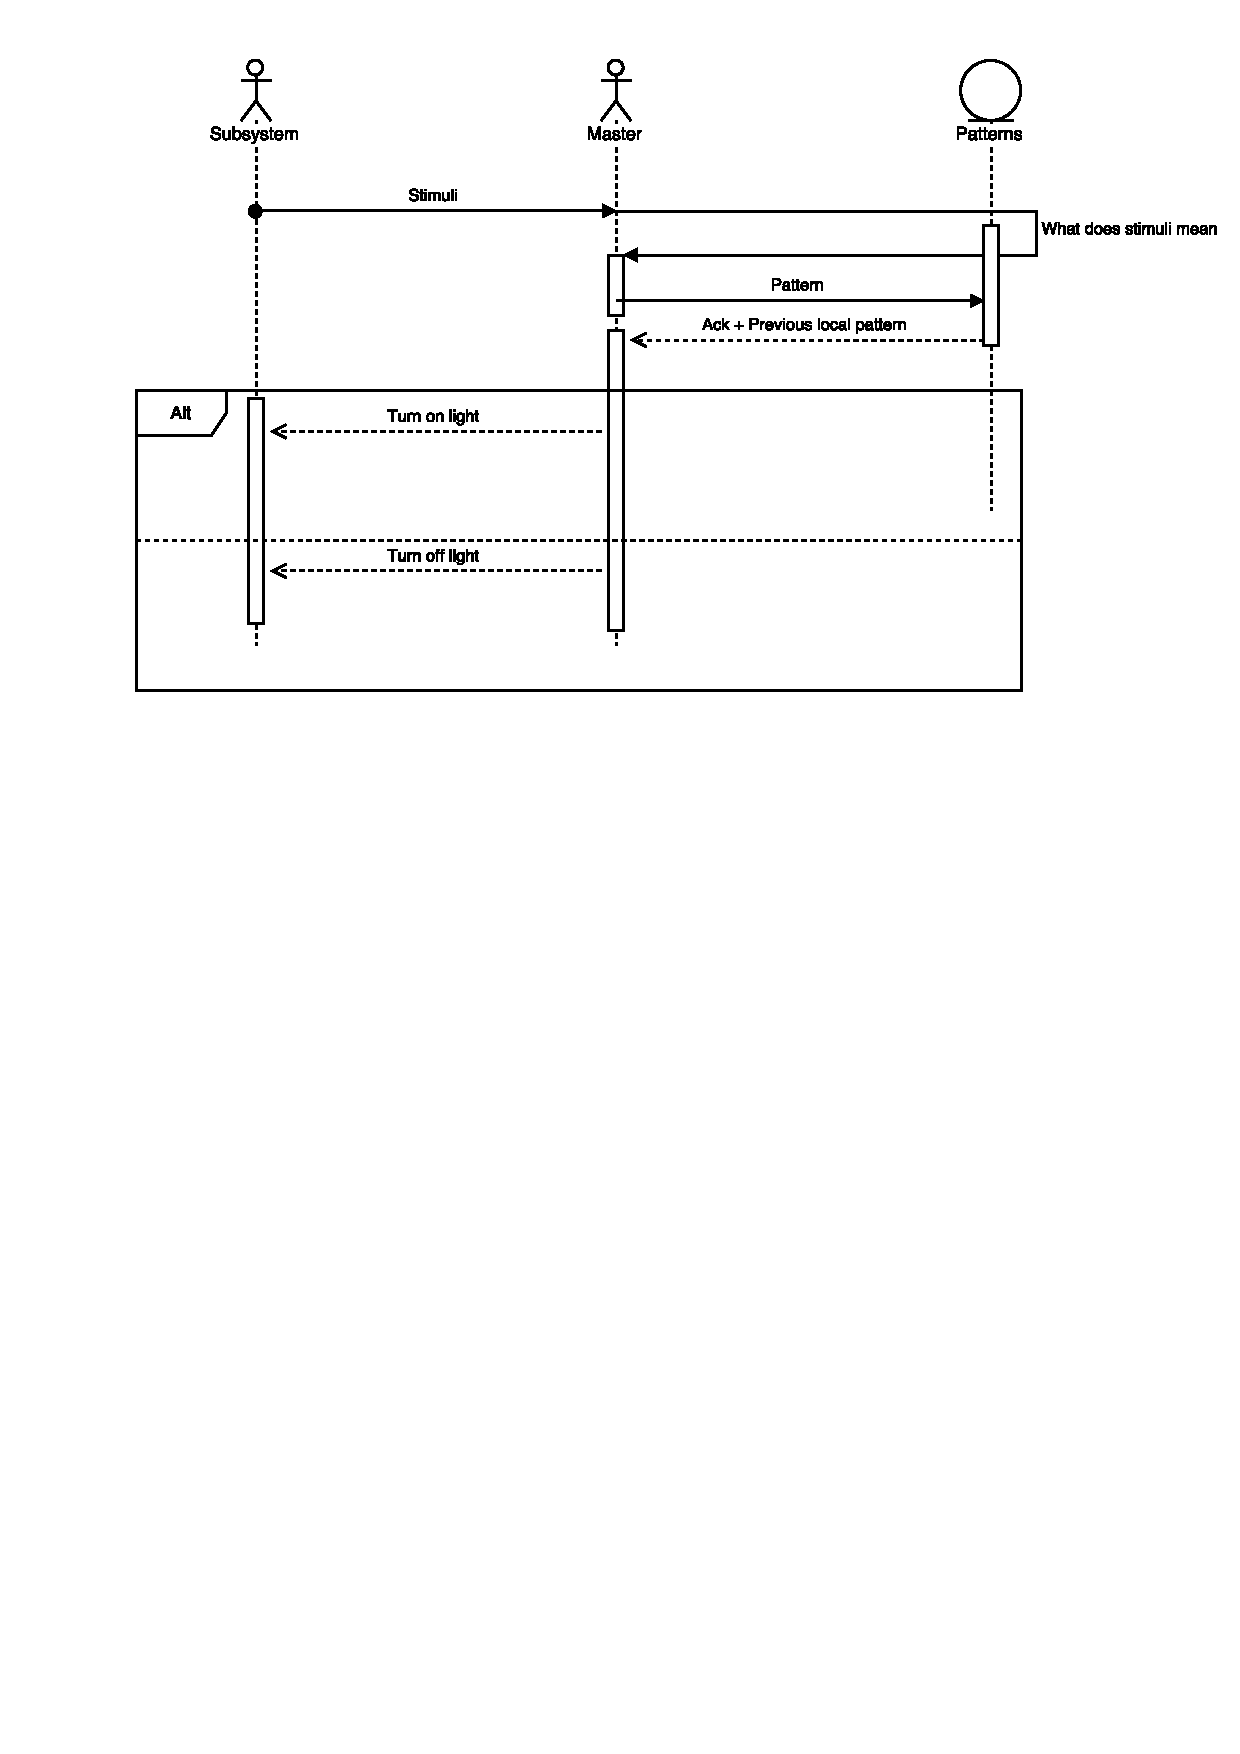
\includegraphics{Behaviour.pdf}
%    \end{adjustbox}
%    \caption{Behaviour diagram}
% \end{figure}
